\documentclass[12pt,a4paper]{article}

\usepackage[utf8]{inputenc}
\usepackage[T1]{fontenc}
\usepackage[english]{babel}
\usepackage{graphicx}
\usepackage{geometry}
\usepackage{fancyhdr}
\usepackage{titlesec}
\usepackage{booktabs}
\usepackage{longtable}
\usepackage{array}
\usepackage{hyperref}
\usepackage{xcolor}
\usepackage{listings}
\usepackage{float}
\usepackage{caption}
\usepackage{subcaption}
\usepackage{amsmath}
\usepackage{enumitem}
\usepackage{tocloft}
\usepackage{tabularx}
\usepackage{geometry}

\geometry{
    left=2.5cm,
    right=2.5cm,
    top=2.5cm,
    bottom=2.5cm
}

\hypersetup{
    colorlinks=true,
    linkcolor=black,
    urlcolor=blue,
    citecolor=black
}

\renewcommand{\lstlistingname}{Code}
\renewcommand{\lstlistlistingname}{List of Codes}
\lstset{
    backgroundcolor=\color{gray!10},
    basicstyle=\ttfamily\scriptsize,
    keywordstyle=\color{blue!70!black}\bfseries,
    commentstyle=\color{green!50!black}\itshape,
    stringstyle=\color{red!70!black},
    breaklines=true,
    breakatwhitespace=false,
    breakautoindent=true,
    postbreak=\mbox{\textcolor{red}{$\hookrightarrow$}\space},
    numbers=left,
    numberstyle=\tiny\color{gray},
    frame=single,
    rulecolor=\color{gray},
    captionpos=b,
    showstringspaces=false,
    tabsize=2,
    columns=flexible,
    keepspaces=true,
    xleftmargin=0.5cm,
    xrightmargin=0.5cm,
    linewidth=\linewidth
}

\pagestyle{fancy}
\fancyhf{}
\fancyhead[L]{\footnotesize INF438 - Advanced Databases}
\fancyhead[R]{\footnotesize Group 3}
\fancyfoot[C]{\thepage}
\renewcommand{\headrulewidth}{0.4pt}
\renewcommand{\footrulewidth}{0.4pt}

\titleformat{\section}
    {\newpage\Large\bfseries}
    {\thesection.}{0.5em}{}
\titleformat{\subsection}
    {\large\bfseries}
    {\thesubsection}{0.5em}{}
\titleformat{\subsubsection}
    {\normalsize\bfseries}
    {\thesubsubsection}{0.5em}{}

\captionsetup[table]{name=Table}

\setcounter{tocdepth}{2}
\renewcommand{\contentsname}{TABLE OF CONTENTS}
\renewcommand{\listfigurename}{LIST OF FIGURES}
\renewcommand{\listtablename}{LIST OF TABLES}

\renewcommand{\arraystretch}{1.2}

\begin{document}

\begin{titlepage}
    \centering
    
    \vspace*{0.5cm}

    \includegraphics[width=5cm, height=5cm, keepaspectratio]{../Screenshots/Picture1}
    
    \vspace{1cm}
    
    {\Large\textbf{GALATASARAY UNIVERSITY}}\\[0.3cm]
    {\large Faculty of Engineering and Technology}\\[0.3cm]
    {\large Department of Computer Engineering}
    
    \vspace{1.5cm}
    
    {\LARGE\textbf{INF438}}\\[0.3cm]
    {\Large\textbf{ADVANCED DATABASES}}
    
    \vspace{1.5cm}
    
    \rule{\textwidth}{1.5pt}\\[0.5cm]
    {\Huge\textbf{Project Final}}\\[0.3cm]
    {\Large E-Sport Analysis (Dota 2) on}\\[0.2cm]
    {\Large Architecture Lakehouse Azure}\\[0.5cm]
    \rule{\textwidth}{1.5pt}
    
    \vspace{1.5cm}
    
    {\large\textbf{GROUP 3}}

    \vspace{0.8cm}

    \begin{tabular}{rl}
        \textbf{Member 1 :} & Sabri Taner Burak ALTINDAL -- 22401030 \\[0.2cm]
        \textbf{Member 2 :} & Emirhan Karatepe -- 19401830 \\[0.2cm]
        \textbf{Member 3 :} & Kaan Çolakoğlu -- 21401946 \\[0.2cm]
        \textbf{Member 4:} & Ceren Akbaş -- 22401028 \\
    \end{tabular}
    
    \vfill
    
    {\large\textbf{Academic Year 2025--2026}}

\end{titlepage}

\newpage
\tableofcontents
\newpage

\listoffigures
\newpage

\listoftables
\newpage

% Section 1: Introduction
\section{Introduction}

\subsection{Project Context}

The e-sports industry has experienced exponential growth over the past decade, becoming a multi-billion dollar ecosystem today. With this growth, the amount of data generated during professional tournaments has also increased significantly. Player performance analysis, team strategy optimization, and match outcome prediction are critical areas where data engineering and data science find practical applications.

As part of this project, a complete data engineering solution was designed and implemented for processing, analyzing, and developing predictive models on professional Dota 2 match data. The project was carried out on the Microsoft Azure platform, adopting modern cloud architecture principles.

\subsection{Dataset Used}

The dataset used in this project is the \textbf{``Dota 2 Pro League Matches 2023''} published on the Kaggle platform. This dataset contains detailed records of professional Dota 2 tournament matches throughout 2023.

\begin{table}[H]
\centering
\caption{Dataset characteristics}
\label{tab:dataset}
\begin{tabular}{>{\centering\arraybackslash}m{4cm}>{\centering\arraybackslash}m{2cm}>{\centering\arraybackslash}m{5cm}}
\toprule
\textbf{File Name} & \textbf{Size} & \textbf{Description} \\
\midrule
main\_metadata.csv & 9.09 MB & Match metadata \\
players\_reduced.csv & 152.00 MB & Player statistics \\
picks\_bans.csv & 33.01 MB & Pick/ban data \\
teams.csv & 8.09 MB & Team information \\
\bottomrule
\end{tabular}
\end{table}

The CSV format and relational structure of the dataset required a complete cleaning and merging process during the transition from the Bronze layer to the Silver layer.

\subsection{Project Objectives}

The main objectives of this project were defined as follows:

\begin{enumerate}[label=\arabic*.]
    \item \textbf{Lakehouse Architecture Setup:} Implementation of the Medallion Architecture (Bronze-Silver-Gold) on Azure Data Lake Storage Gen2
    \item \textbf{Batch Processing Pipeline:} Creation of automated ETL pipelines using Azure Data Factory and Databricks
    \item \textbf{Streaming Simulation:} Development of a simulator mimicking real-time data flow
    \item \textbf{Data Transformation:} Transformation of raw data into analytical tables using PySpark
    \item \textbf{Advanced Analysis:} Player and hero performance analyses with SQL and PySpark
    \item \textbf{Machine Learning:} Development of a match outcome prediction model and tracking with MLflow
\end{enumerate}

\subsection{Azure Services Used}

\begin{table}[H]
\centering
\caption{Microsoft Azure services used}
\label{tab:azure-services}
\begin{tabular}{>{\centering\arraybackslash}m{5cm}>{\centering\arraybackslash}m{7cm}}
\toprule
\textbf{Service} & \textbf{Usage Purpose} \\
\midrule
Azure Data Lake Storage Gen2 & Central storage for Lakehouse layers \\
Azure Data Factory & Pipeline orchestration and scheduling \\
Azure Databricks & Data processing and ML development \\
Delta Lake & High-performance ACID-compliant data format \\
MLflow & Machine learning experiment tracking \\
Power BI & Visualization and dashboard creation \\
\bottomrule
\end{tabular}
\end{table}

All resources were created using the \textbf{Microsoft Azure for Students} subscription and managed with cost optimization in mind.

% Section 2: Architectural Design
\section{Architectural Design}

\subsection{Medallion Architecture}

In this project, the \textbf{Medallion Architecture}, widely adopted in modern data engineering practices, was applied. This architecture divides data into three layers according to their level of quality and processing: \textbf{Bronze}, \textbf{Silver}, and \textbf{Gold}.

\subsubsection{Bronze Layer (Raw Data)}

The Bronze layer is where data from source systems is stored as-is, without any transformation:

\begin{itemize}
    \item \textbf{Purpose:} Preserving an exact copy of the data source
    \item \textbf{Format:} CSV and JSON (for streaming simulation)
    \item \textbf{Content:} 4 main CSV files + streaming JSON files
    \item \textbf{Usage:} Return to source in case of error, audit and traceability
\end{itemize}


\subsubsection{Silver Layer (Cleaned Data)}

The Silver layer is the intermediate layer where raw data is cleaned and standardized:

\begin{itemize}
    \item \textbf{Purpose:} Provide clean and consistent data
    \item \textbf{Format:} Delta Lake (Parquet-based)
    \item \textbf{Transformations:} Null value cleaning, type standardization, duplicate elimination, outlier detection
\end{itemize}

\begin{table}[H]
\centering
\caption{Silver layer tables}
\label{tab:silver-tables}
\begin{tabular}{>{\centering\arraybackslash}m{5cm}>{\centering\arraybackslash}m{5cm}}
\toprule
\textbf{Table} & \textbf{Number of Records} \\
\midrule
cleaned\_matches & 29 809 \\
cleaned\_players & 8 456 \\
cleaned\_picks\_bans & 710 414 \\
\bottomrule
\end{tabular}
\end{table}

\subsubsection{Gold Layer (Analytical Data)}

The Gold layer contains data enriched with business logic:

\begin{table}[H]
\centering
\caption{Gold layer tables}
\label{tab:gold-tables}
\begin{tabular}{>{\centering\arraybackslash}m{4.5cm}>{\centering\arraybackslash}m{4.5cm}>{\centering\arraybackslash}m{3cm}}
\toprule
\textbf{Table} & \textbf{Description} & \textbf{Records} \\
\midrule
esports\_gold.player\_stats & Performance metrics & 813 \\
esports\_gold.hero\_stats & Hero statistics & 123 \\
esports\_gold.daily\_stats & Daily statistics & 365 \\
esports\_gold.ml\_features & ML features & 8 312 \\
\bottomrule
\end{tabular}
\end{table}

\subsection{Azure Data Lake Storage Gen2 Structure}

All Lakehouse layers are positioned on Azure Data Lake Storage Gen2:

\begin{itemize}
    \item \textbf{Storage Account:} \texttt{dota2lakehousenew}
    \item \textbf{Container:} \texttt{data}
    \item \textbf{Paths:}
    \begin{itemize}
        \item Bronze: \texttt{abfss://data@dota2lakehousenew.../bronze/}
        \item Silver: \texttt{abfss://data@dota2lakehousenew.../silver/}
        \item Gold: \texttt{abfss://data@dota2lakehousenew.../gold/}
    \end{itemize}
\end{itemize}

\begin{figure}[H]
\centering
\includegraphics[width=\textwidth, height=0.75\textheight, keepaspectratio]{../Screenshots/Picture2}
\caption{Azure Portal view of Bronze/Silver/Gold folder structure in ADLS Gen2}
\label{fig:adls-structure}
\end{figure}

\subsection{Data Flow Diagram}

The end-to-end data flow of the system follows this path: source data from Kaggle and the streaming simulator is first stored in the Bronze layer. Then, Azure Data Factory orchestrates the Databricks notebooks that transform data to the Silver and then Gold layers. Finally, Gold data feeds SQL analytics, the machine learning model (tracked by MLflow), and Power BI visualizations.

\begin{figure}
    \centering
    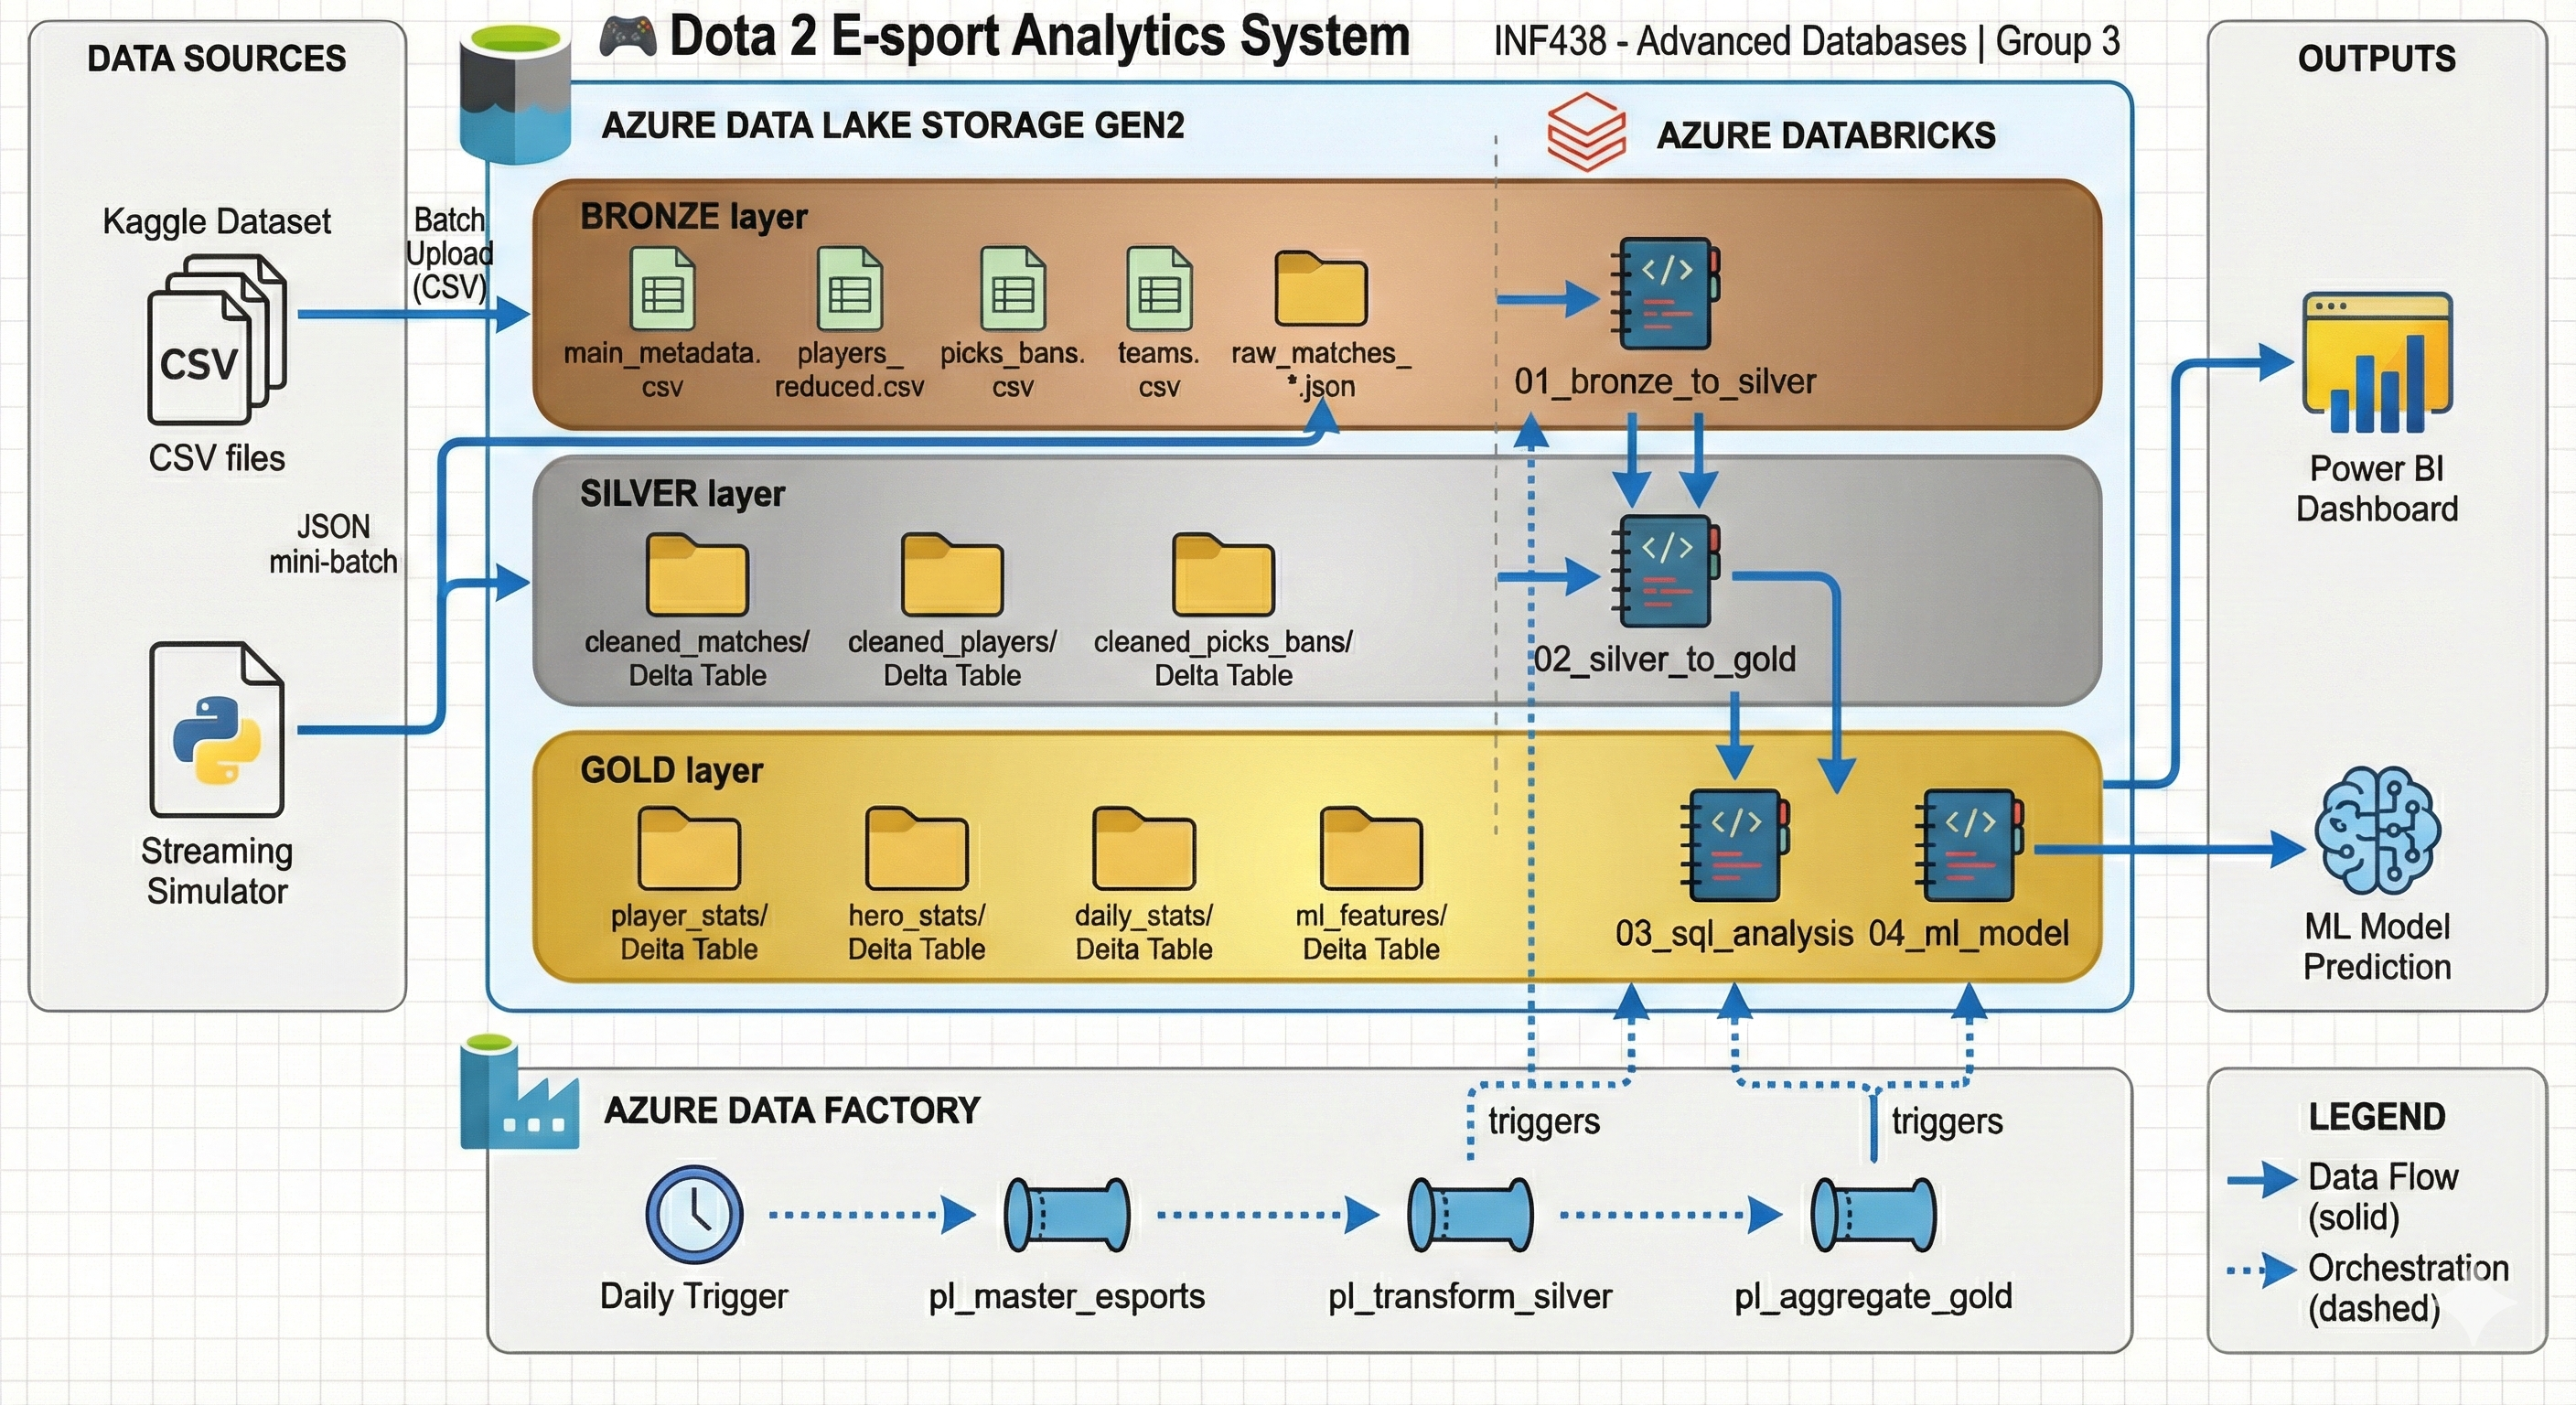
\includegraphics[width=0.60\linewidth]{../Screenshots/pipeline.png}
    \caption{Data flow diagram}
    \label{fig:placeholder}
\end{figure}

% Section 3: Implementation
\section{Implementation}

\subsection{Batch Processing Pipeline}

Azure Data Factory (ADF) was used for batch processing pipeline orchestration. The main pipeline created in the project is named \textbf{pl\_master\_esports}.

Upstream of this processing, a specific ingestion pipeline named \\\texttt{PL\_Ingest\_Kaggle\_To\_Bronze} was set up. This pipeline uses a \textit{Copy Data} activity to automatically transfer raw files (CSV) and the reduced dataset to the \texttt{bronze/} container of the Data Lake, ensuring data availability for Databricks notebooks.

\begin{figure}[H]
\centering
\includegraphics[width=\textwidth, height=0.75\textheight, keepaspectratio]{../Screenshots/batch_pipeline.png}
\caption{Execution details of the \textit{Copy Data} activity confirming successful ingestion of 4 source files (212 MB) to the Bronze container.}
\label{fig:adf-pipeline}
\end{figure}

The pipeline structure is designed as follows:
\begin{itemize}
    \item \textbf{Activity 1:} nb\_bronze\_to\_silver (Databricks Notebook)
    \item \textbf{Activity 2:} nb\_silver\_to\_gold (depends on Activity 1)
    \item \textbf{Activity 3:} nb\_ml\_model (depends on Activity 2)
\end{itemize}

\begin{figure}[H]
\centering
\includegraphics[width=\textwidth, height=0.75\textheight, keepaspectratio]{../Screenshots/Picture3}
\caption{pl\_master\_esports pipeline diagram in Azure Data Factory}
\label{fig:adf-pipeline}
\end{figure}

\subsection{Trigger Configuration}

A trigger named \textbf{tr\_daily\_esports} was created for automatic pipeline execution.

\begin{table}[H]
\centering
\caption{Trigger configuration}
\label{tab:trigger-config}
\begin{tabular}{>{\centering\arraybackslash}m{4cm}>{\centering\arraybackslash}m{5cm}}
\toprule
\textbf{Parameter} & \textbf{Value} \\
\midrule
Trigger Name & tr\_daily\_esports \\
Type & Schedule Trigger \\
Frequency & Daily \\
Start Time & 02:00 UTC \\
Status & Active \\
\bottomrule
\end{tabular}
\end{table}

\begin{figure}[H]
\centering
\includegraphics[width=\textwidth, height=0.75\textheight, keepaspectratio]{../Screenshots/Picture4}
\caption{``Succeeded'' status and ``Triggered by tr\_daily\_esports'' in the ADF Monitor screen}
\label{fig:adf-monitor}
\end{figure}

\subsection{Databricks Notebooks}

Data transformation operations were performed using PySpark on Azure Databricks.

\begin{table}[H]
\centering
\caption{Databricks cluster configuration}
\label{tab:cluster-config}
\begin{tabular}{>{\centering\arraybackslash}m{4cm}>{\centering\arraybackslash}m{5cm}}
\toprule
\textbf{Parameter} & \textbf{Value} \\
\midrule
Cluster Mode & Standard \\
Node Type & Standard\_DS3\_v2 \\
Auto Termination & 120 minutes \\
Databricks Runtime & 13.3 LTS (Spark 3.4.1) \\
\bottomrule
\end{tabular}
\end{table}

\textbf{Notebooks created:}
\begin{enumerate}
    \item \textbf{setup\_connection.ipynb}: Azure ADLS Gen2 connection test
    \item \textbf{01\_bronze\_to\_silver.ipynb}: Raw data cleaning
    \item \textbf{02\_silver\_to\_gold.ipynb}: Business logic application
    \item \textbf{04\_ml\_model.ipynb}: ML model training
\end{enumerate}

The complete source code of these notebooks is available in \textbf{Appendix~\ref{appendix:notebooks}}.

\subsection{Streaming Simulation}

In the absence of a real-time data source, a Python script simulating streaming behavior was developed. The \textbf{stream\_simulator.py} script operates according to the following logic:

\begin{enumerate}
    \item Records are read from the main\_metadata.csv file
    \item Records are divided into mini-batches of 5
    \item An artificial delay of 3 seconds is applied for each mini-batch
    \item The mini-batch is named with a unique timestamp and written to Bronze
\end{enumerate}

\begin{figure}[H]
\centering
\includegraphics[width=\textwidth, height=0.75\textheight, keepaspectratio]{../Screenshots/simulation-streaming.png}
\caption{stream\_simulator.py execution output}
\label{fig:stream-output}
\end{figure}

When the simulator is executed, files are created in the Bronze layer with the format \texttt{raw\_matches\_YYYYMMDD\_HHMMSS.json} (10 files in total).

The complete source code of the simulator is available in \textbf{Appendix~\ref{appendix:streaming}}.

\subsection{ETL Transformations}

\subsubsection{Bronze → Silver Transformation}

The raw CSV data from the Bronze layer underwent a complete transformation process:

\begin{itemize}
    \item \textbf{Loading:} Reading CSV files with schema inference
    \item \textbf{Cleaning:} Removing unnecessary columns, filtering null values
    \item \textbf{Validation:} Filtering matches with invalid duration ($<$5 min or $>$2 hours)
    \item \textbf{Enrichment:} Creating new features (duration\_minutes, kda\_calculated)
    \item \textbf{Outlier Detection:} Marking using the 3-sigma rule
\end{itemize}

\subsubsection{Silver → Gold Transformation}

The cleaned data received business logic and advanced calculations.

\textbf{Player Statistics (player\_stats):} Aggregation by player account with calculation of averages (KDA, GPM, XPM) and win rate. Result: statistics calculated for \textbf{813 unique players}.

\textbf{Hero Meta Analysis (hero\_stats):} A classification algorithm for heroes into 5 tiers according to their presence rate (see Table~\ref{tab:tier-criteria}).

\begin{table}[H]
\centering
\caption{Meta Tier classification criteria}
\label{tab:tier-criteria}
\begin{tabular}{>{\centering\arraybackslash}m{3cm}>{\centering\arraybackslash}m{5cm}}
\toprule
\textbf{Tier} & \textbf{Presence Rate Criterion} \\
\midrule
S-Tier & $>$ 50\% \\
A-Tier & $>$ 30\% \\
B-Tier & $>$ 15\% \\
C-Tier & $>$ 5\% \\
D-Tier & $\leq$ 5\% \\
\bottomrule
\end{tabular}
\end{table}

\begin{figure}[H]
\centering
\includegraphics[width=\textwidth, height=0.75\textheight, keepaspectratio]{../Screenshots/Picture6}
\caption{Tier classification output in silver\_to\_gold notebook}
\label{fig:tier-classification}
\end{figure}

\textbf{Match Duration Analysis:}

\begin{table}[H]
\centering
\caption{Duration analysis results}
\label{tab:duration-analysis}
\begin{tabular}{>{\centering\arraybackslash}m{3.5cm}>{\centering\arraybackslash}m{2cm}>{\centering\arraybackslash}m{2cm}>{\centering\arraybackslash}m{2.5cm}}
\toprule
\textbf{Duration} & \textbf{Matches} & \textbf{Avg Kills} & \textbf{Radiant Win} \\
\midrule
Very Short ($<$25min) & 4 176 & 44.94 & 53.54\% \\
Short (25-35min) & 13 548 & 56.74 & 50.41\% \\
Medium (35-45min) & 8 162 & 65.33 & 49.36\% \\
Long (45-55min) & 2 839 & 68.19 & 49.52\% \\
Very Long ($>$55min) & 1 084 & 80.77 & 50.46\% \\
\bottomrule
\end{tabular}
\end{table}

\subsection{Delta Lake Table Management}

The Gold layer tables are managed under the \textbf{esports\_gold} schema in the Databricks Unity Catalog. The SQL creation commands are available in \textbf{Appendix~\ref{appendix:sql}}.

\begin{figure}[H]
\centering
\includegraphics[width=\textwidth, height=0.75\textheight, keepaspectratio]{../Screenshots/Picture7}
\caption{List of tables under esports\_gold schema in Databricks Catalog}
\label{fig:catalog-tables}
\end{figure}

% Section 4: Analysis and ML
\section{Data Analysis and Machine Learning}

\subsection{Accessing Gold Tables and SQL Execution (Databricks)}

\subsubsection{Connection to Azure Data Lake Storage (ADLS Gen2)}

The analytical tables of the \textit{Gold} layer are stored on Azure Data Lake Storage Gen2 in Delta Lake format. 
In our case, certain limitations of the \textit{Azure for Students} subscription (quotas / RBAC permissions) prevented direct and stable access for all group members. 
To ensure project continuity, access to the \textit{Storage Account} was done via an access key provided by a group member with the necessary permissions. 
This key is never exposed in the report or in plain text in versioned code; it is injected via Databricks environment variables.

\paragraph{CPU constraints and use of a shared cluster.}
During notebook execution with the Azure for Students subscription, we encountered resource limitations (CPU/vCore quota) and slowdowns that could interrupt certain Spark processing tasks.
To avoid deadlocks and complete the work on time, we used the Databricks cluster already configured by a group member (esports-cluster), which had more stable resources (16 GB RAM and 4 cores).
Thanks to this solution, we were able to correctly execute ETL transformations, access Delta tables in the Gold layer, and run analytical SQL queries without interruptions.



\subsubsection{Loading Gold Tables and Creating Temporary Views}

To execute SQL queries directly on Delta files in the Gold layer, we loaded each table from ADLS and created temporary views in Databricks.

\begin{figure}[H]
\centering
\includegraphics[width=\textwidth]{../Screenshots/gold_tables_created.png}
\caption{Loading Gold tables from ADLS Gen2 and creating temporary views in Databricks}
\label{fig:gold-tables-created}
\end{figure}

\subsection{Analytical SQL Queries (Results)}

This section presents the main SQL queries used to produce analyses on players, heroes, and daily activity. 
To keep the report readable, we present here the outputs (screenshots); complete queries can be added in the appendix if needed.

\subsubsection{Top 10 Players by Performance (KDA)}

Objective: identify the 10 most performing players according to their average KDA (with filtering to avoid non-representative cases).

\begin{figure}[H]
\centering
\includegraphics[width=\textwidth]{../Screenshots/player_top10_avg_kda_total_kills_deaths_assists.png}
\caption{SQL Result: Top 10 players by average KDA (with kills, deaths, assists)}
\label{fig:sql-top10-players-kda}
\end{figure}

\subsubsection{Daily Trends: Match Volume and Average Duration}

Objective: observe the daily evolution of the number of matches as well as the average duration (conversion to minutes).

\begin{figure}[H]
\centering
\includegraphics[width=\textwidth]{../Screenshots/Last10DaysSummary.png}
\caption{SQL Result: daily statistics overview (match\_count and average duration in minutes)}
\label{fig:sql-daily-trends}
\end{figure}

\subsubsection{Top 10 Heroes: Economic Performance (GPM/XPM)}

Objective: identify heroes with the best economic performance via \texttt{avg\_gpm} and \texttt{avg\_xpm}.

\begin{figure}[H]
\centering
\includegraphics[width=\textwidth]{../Screenshots/hero_top10_avg_gpm_avg_xpm.png}
\caption{SQL Result: Top 10 heroes by average GPM and XPM}
\label{fig:sql-top10-hero-gpm-xpm}
\end{figure}

\subsubsection{Top 10 Heroes: Combat Style (Kills/Assists)}

Objective: analyze the most aggressive heroes via the \texttt{avg\_kills} and \texttt{avg\_assists} metrics, taking into account the volume (\texttt{times\_played}).

\begin{figure}[H]
\centering
\includegraphics[width=\textwidth]{../Screenshots/hero_top10_avg_kills_avg_assists_times_played.png}
\caption{SQL Result: Top 10 combat-oriented heroes (kills/assists) and number of games played}
\label{fig:sql-top10-hero-combat}
\end{figure}

\subsubsection{Top 10 Most Popular Heroes}

Objective: identify the most played heroes based on the number of appearances (times played). 
We also display the number of wins and win rate (in \%).

\begin{figure}[H]
\centering
\includegraphics[width=\textwidth]{../Screenshots/Top10Kahraman.png}
\caption{SQL Result: Top 10 most popular heroes by times\_played (with wins and win\_rate)}
\label{fig:sql-top10-heroes-picks}
\end{figure}


The analysis reveals that in very short matches ($<$25 min), the Radiant team has a slight advantage (53.54\%). This rate balances around 50\% for longer matches.

\subsection{Power BI Visualization}
\subsubsection{Connection and Data Loading in Power BI}

We performed the visualization part with Power BI Desktop using Gold data. 
To retrieve the data, we used \textit{Get Data} then the \textit{Azure Blob Storage} source. 
Since not everyone could connect easily (rights/quotas Azure for Students), we used an access key shared by a group member.

After connecting, we found the Parquet files in the \textit{data} container (Gold layer) and imported the tables \textit{daily\_stats}, \textit{player\_stats}, \textit{hero\_stats}, and \textit{ml\_features}. 
Then, we added a \textit{Date} table to filter by time, and linked it to \textit{daily\_stats} with the \textit{match\_date} column. 
Finally, we created the pages and charts to analyze overall trends, top players, and hero meta.


\subsubsection{Page 1: Overview and Daily Trends}

This page provides a quick reading of 2023 activity:
(i) a date slicer that controls all indicators,
(ii) a daily trend of the number of matches,
(iii) KPI cards: total number of matches, average Radiant win rate, and average match duration.

\textbf{Observations.}
We observe relatively stable activity over a large part of the year, with daily fluctuations.
A marked peak appears during a specific period (end of year), which may correspond to an event (tournament, major patch, or high competitive activity).
The average Radiant win rate remains close to balance, suggesting no lasting systematic advantage over the year.
The average match duration is generally stable, with occasional variations indicating changes in play style or meta.

\begin{figure}[H]
\centering
\includegraphics[width=\textwidth]{../Screenshots/pbi_overview_daily_trends.png}
\caption{Power BI --- Overview Page: temporal filter, daily trend of match count, and global KPIs}
\label{fig:pbi-overview}
\end{figure}

\subsubsection{Page 2: Top 10 Players}

This page compares players according to:
(i) Top 10 players by average KDA,
(ii) Top 10 players by win rate,
with a detailed table of statistics (matches, wins, KDA, XPM, etc.).

\textbf{Observations.}
The KDA ranking highlights profiles oriented towards individual performance (survival + combat efficiency).
The win rate ranking is not necessarily identical: a player may have a high KDA but a more moderate win rate, highlighting the importance of teamwork and match context.
The table allows verifying result consistency by simultaneously comparing match volume and indicators, and avoiding over-interpreting players with too few games.

\begin{figure}[H]
\centering
\includegraphics[width=\textwidth]{../Screenshots/pbi_top10_players.png}
\caption{Power BI --- Top 10 Players Page: average KDA vs win rate comparison and detail table}
\label{fig:pbi-top10-players}
\end{figure}

\subsubsection{Page 3: Hero Meta Analysis}

This page is dedicated to the meta:
(i) a scatter plot linking \textit{presence\_rate} and \textit{win\_rate} by hero,
(ii) a Top 10 of the most present heroes.

\textbf{Observations.}
The scatter plot highlights several interesting zones:
\begin{itemize}
  \item very present heroes but with an average win rate: often "meta" or flexible picks, not necessarily dominant;
  \item less present heroes but with a high win rate: "underrated" candidates or very effective situational picks;
  \item present and performing heroes: they constitute the dominant meta and deserve special attention.
\end{itemize}
The Top 10 of the most present heroes synthesizes popularity and facilitates identification of heroes played most frequently over the filtered period.

\begin{figure}[H]
\centering
\includegraphics[width=\textwidth]{../Screenshots/pbi_hero_meta.png}
\caption{Power BI --- Hero Meta Page: presence rate vs win rate relationship and Top 10 most present heroes}
\label{fig:pbi-hero-meta}
\end{figure}

\subsubsection{Page 4: Match Duration and Correlations}

This page analyzes:
(i) the temporal evolution of average match duration,
(ii) the relationship between duration and intensity (e.g., average kills) via a scatter plot.

\textbf{Observations.}
The average duration varies within a relatively limited range, but certain lows/peaks suggest periods where matches end more quickly (aggressive strategies) or conversely lengthen (more controlled games).
The duration vs kills scatter plot shows a globally weak to moderate relationship: longer matches tend to offer more combat opportunities, but dispersion indicates that other factors strongly influence the number of kills (level gap, drafts, team styles).
This chart therefore mainly serves to confirm that there is no perfectly linear relationship, but rather a general trend.

\begin{figure}[H]
\centering
\includegraphics[width=\textwidth]{../Screenshots/pbi_duration_correlation.png}
\caption{Power BI --- Duration and Correlations Page: average duration trend and duration vs kills correlation}
\label{fig:pbi-duration-corr}
\end{figure}



\subsection{Machine Learning Model}

A binary classification model was developed to predict match outcome. The target variable is \texttt{win} (1 = Win, 0 = Loss).

\begin{table}[H]
\centering
\caption{Features used}
\label{tab:features}
\begin{tabular}{>{\centering\arraybackslash}m{3.5cm}>{\centering\arraybackslash}m{5cm}>{\centering\arraybackslash}m{3cm}}
\toprule
\textbf{Feature} & \textbf{Description} & \textbf{Category} \\
\midrule
kills & Number of kills & Combat \\
deaths & Number of deaths & Combat \\
assists & Number of assists & Combat \\
gold\_per\_min & Gold per minute & Economy \\
xp\_per\_min & Experience per minute & Economy \\
hero\_damage & Hero damage & Damage \\
tower\_damage & Tower damage & Damage \\
last\_hits & Number of last hits & Progression \\
level & Player level & Progression \\
duration\_minutes & Match duration & Match Info \\
\bottomrule
\end{tabular}
\end{table}

The \textbf{Random Forest Classifier} algorithm was chosen with parameters: numTrees=50, maxDepth=10, Train/Test Split=80\%/20\%.

The complete ML pipeline source code is available in \textbf{Appendix~\ref{appendix:ml}}.

\subsection{Model Results}

\begin{center}
\fbox{
\begin{minipage}{0.7\textwidth}
\centering
\vspace{0.5cm}
\textbf{\large MODEL RESULTS}\\[0.5cm]
\rule{0.9\textwidth}{0.5pt}\\[0.3cm]
Model used: \textbf{Random Forest Classifier}\\[0.3cm]
Accuracy: \textbf{\LARGE 87.34\%}\\[0.3cm]
\rule{0.9\textwidth}{0.5pt}
\vspace{0.5cm}
\end{minipage}
}
\end{center}

\begin{table}[H]
\centering
\caption{Confusion Matrix}
\label{tab:confusion-matrix}
\begin{tabular}{>{\centering\arraybackslash}m{3cm}|>{\centering\arraybackslash}m{2.5cm}>{\centering\arraybackslash}m{2.5cm}}
\toprule
\textbf{Actual / Predicted} & \textbf{Lose (0)} & \textbf{Win (1)} \\
\midrule
\textbf{Lose (0)} & 727 (TN) & 131 (FP) \\
\textbf{Win (1)} & 81 (FN) & 735 (TP) \\
\bottomrule
\end{tabular}
\end{table}

\textbf{Calculated metrics:}
\begin{itemize}
    \item True Positive Rate (Recall): $\frac{735}{735+81} = 90.07\%$
    \item True Negative Rate: $\frac{727}{727+131} = 84.73\%$
    \item Precision: $\frac{735}{735+131} = 84.87\%$
\end{itemize}

\subsection{Feature Importance Analysis}

\begin{table}[H]
\centering
\caption{Feature importance ranking}
\label{tab:feature-importance}
\begin{tabular}{>{\centering\arraybackslash}m{2cm}>{\centering\arraybackslash}m{4cm}>{\centering\arraybackslash}m{4cm}}
\toprule
\textbf{Rank} & \textbf{Feature} & \textbf{Importance} \\
\midrule
1 & assists & 0.311480 \\
2 & deaths & 0.204537 \\
3 & tower\_damage & 0.147192 \\
4 & xp\_per\_min & 0.073274 \\
5 & last\_hits & 0.058863 \\
6 & duration\_minutes & 0.049268 \\
7 & gold\_per\_min & 0.048150 \\
8 & kills & 0.040887 \\
9 & hero\_damage & 0.040081 \\
10 & level & 0.026267 \\
\bottomrule
\end{tabular}
\end{table}

These results show that \textbf{teamwork} (\texttt{assists} with 0.311) is the most determining factor on match outcome, followed by \textbf{survival} (\texttt{deaths} with 0.205) and \textbf{objective damage} (\texttt{tower\_damage} with 0.147).
 
Contrary to expectations, economic factors (\texttt{gold\_per\_min}: 0.048, \texttt{xp\_per\_min}: 0.073) have relatively low importance. This suggests that in professional Dota 2 matches, team coordination and objective-oriented play are more predictive of victory than individual resource accumulation.

\subsection{MLflow Tracking}

All model experiments were automatically tracked on MLflow with \texttt{mlflow.autolog()}.

\begin{figure}[H]
\centering
\includegraphics[width=\textwidth, height=0.75\textheight, keepaspectratio]{../Screenshots/Picture9}
\caption{Model results and parameters in MLflow interface}
\label{fig:mlflow-results}
\end{figure} 
% Section 5: Challenges and Solutions
\section{Challenges Encountered and Solutions}

\subsection{Azure Resource Limitations}

\textbf{Problem:} The Azure for Students subscription contains strict resource limits (notably vCore quota and limited credits).

\textbf{Solution:} Cluster size was kept to minimum (Standard\_DS3\_v2), auto-termination time was set to 120 minutes, and the cluster was manually stopped after operations to save credits.

\subsection{File Collisions in Streaming Simulation}

\textbf{Problem:} During rapid simulation script execution, multiple mini-batches could be created within the same second, causing file name collisions and data overwrites.

\textbf{Solution:} A delay of \texttt{SLEEP\_TIME = 3} seconds was added in the ingestion loop. Additionally, file names now use a precise timestamp in \texttt{YYYYMMDD\_HHMMSS} format.

\subsection{Data Volume and Cost Constraints}

\textbf{Problem:} The original source file \texttt{players.csv} exceeded 5.3 GB. Processing this complete volume would have quickly exhausted Azure credits and the available student cluster computing capacity.

\textbf{Solution:} Local pre-processing was performed to generate a representative \texttt{players\_reduced.csv} file (152 MB). We then used Delta Lake format to optimize read/write performance on this reduced dataset.

\subsection{Azure Storage Key Management}

\textbf{Problem:} The storage account key needed to be shared between developers and services without being exposed in plain text in code.

\textbf{Solution:} Use of environment variables (\texttt{AZURE\_STORAGE\_KEY}), secure storage with Databricks secrets, and local development with \texttt{.env} file.

\subsection{Access Management Complexity (IAM)}

\textbf{Problem:} Team collaboration caused recurring permission issues (IAM). Assigning the "Contributor" role was not sufficient for certain actions (such as reading Blob data or accessing Cost Management), which caused significant delays in time management and project progress.

\textbf{Solution:} A more granular RBAC strategy was adopted, explicitly assigning \textit{Storage Blob Data Owner} and \textit{Cost Management Contributor} roles to appropriate members via the Azure portal.

\newpage
\subsection{Databricks Cluster Access Issues}

\textbf{Problem:} Due to limitations of the \textit{Azure for Students} subscription, I could not create or select a Databricks cluster, which prevented notebook execution and thus launching SQL analyses on Gold data.

\textbf{Solution:} To ensure project progress, a group member with the necessary permissions temporarily delegated access to their Databricks cluster (\textit{esports-cluster}). This allowed me to execute SQL queries on Gold tables and continue the analytical phase. Access information was not exposed in plain text: the key and connection parameters were managed securely via Databricks environment variables and \textit{Databricks Secrets}.

% Section 6: Conclusion
\section{Conclusion}

\subsection{Project Summary}

This project demonstrated how modern data engineering concepts (Lakehouse, Delta Lake, MLOps) can be applied in a practical e-sports scenario.

\begin{table}[H]
\centering
\caption{Main results obtained}
\label{tab:results-summary}
\begin{tabular}{>{\centering\arraybackslash}m{4cm}>{\centering\arraybackslash}m{8cm}}
\toprule
\textbf{Component} & \textbf{Result} \\
\midrule
Medallion Architecture & Bronze/Silver/Gold layers implemented \\
Data Processing & 29 809 matches, 8 456 players processed \\
Streaming Simulation & 10 mini-batches written to Bronze \\
Gold Tables & 4 analytical tables (813 players, 123 heroes) \\
ML Model & Random Forest with 87.34\% accuracy \\
Meta Analysis & Classification of heroes into 5 tiers \\
\bottomrule
\end{tabular}
\end{table}

\subsection{Lessons Learned}

\begin{itemize}
    \item \textbf{Cloud Resource Management:} Azure cost and resource optimization
    \item \textbf{Delta Lake Benefits:} ACID transactions, schema evolution, performance
    \item \textbf{Orchestration:} Management of complex flows with Azure Data Factory
    \item \textbf{MLOps Best Practices:} Importance of tracking experiments with MLflow
\end{itemize}

\subsection{General Conclusion}

The integrated services offered by the Azure ecosystem enabled rapid and efficient development of an end-to-end data solution. The ML model with an accuracy rate of \textbf{87.34\%} proved that player performance metrics can predict match outcome with high precision. In particular, teamwork and objective-focused features (\texttt{assists}, \texttt{tower\_damage}) were identified as the most determining characteristics.

\newpage
\appendix
\section*{APPENDICES}
\addcontentsline{toc}{section}{Appendices}

\subsection*{Databricks Notebooks Source Code}
\label{appendix:notebooks}

\subsubsection*{setup\_connection.ipynb}

\begin{lstlisting}[language=Python, caption=Azure ADLS Gen2 connection test]
# Notebook: setup_connection
import os

storage_account = "dota2lakehousenew"
container = "data"
storage_account_key = os.environ.get("AZURE_STORAGE_KEY")
print(f"Key loaded: {storage_account_key is not None}")

spark.conf.set(
  f"fs.azure.account.key.{storage_account}.dfs.core.windows.net",
  storage_account_key)

BRONZE = f"abfss://{container}@{storage_account}.dfs.core.windows.net/bronze"
SILVER = f"abfss://{container}@{storage_account}.dfs.core.windows.net/silver"
GOLD = f"abfss://{container}@{storage_account}.dfs.core.windows.net/gold"

print("=== Files in Bronze Layer ===")
for f in dbutils.fs.ls(BRONZE):
  print(f"  {f.name} ({f.size/1024/1024:.2f} MB)")
\end{lstlisting}

\subsubsection*{01\_bronze\_to\_silver.ipynb (Extraits)}

\begin{lstlisting}[language=Python, caption=Data loading and cleaning]
from pyspark.sql.functions import *
df_matches = spark.read.csv(f"{BRONZE}/main_metadata.csv",
  header=True, inferSchema=True)
df_players = spark.read.csv(f"{BRONZE}/players_reduced.csv",
  header=True, inferSchema=True)
df_matches_clean = df_matches \
  .drop("Unnamed: 0").dropDuplicates(["match_id"]) \
  .filter(col("match_id").isNotNull()) \
  .filter((col("duration") > 300) & (col("duration") < 7200))
df_matches_clean = df_matches_clean \
  .withColumn("duration_minutes", round(col("duration")/60, 2)) \
  .withColumn("radiant_win", col("radiant_win").cast("boolean")) \
  .withColumn("match_date", to_date(col("start_date_time")))
stats = df_players.select(
  mean("kills").alias("m"), stddev("kills").alias("s")).collect()[0]
df_players = df_players.withColumn("is_outlier",
  when(col("kills") > stats["m"] + 3*stats["s"], True).otherwise(False))
df_matches_clean.write.format("delta").mode("overwrite") \
  .save(f"{SILVER}/cleaned_matches")
\end{lstlisting}

\subsubsection*{02\_silver\_to\_gold.ipynb (Extraits)}

\begin{lstlisting}[language=Python, caption=Gold tables creation]
df_player_stats = df_players \
  .filter(col("account_id").isNotNull()) \
  .groupBy("account_id").agg(
    count("match_id").alias("total_matches"),
    sum("win").alias("total_wins"),
    round(avg("kills"), 2).alias("avg_kills"),
    round(avg("kda_calculated"), 2).alias("avg_kda"),
    round(avg("gold_per_min"), 2).alias("avg_gpm")) \
  .withColumn("win_rate",
    round(col("total_wins")/col("total_matches")*100, 2))
total = df_matches.count()
df_hero = df_hero \
  .withColumn("presence_rate", 
    round(col("total_presence")/(total*2)*100, 2)) \
  .withColumn("meta_tier",
    when(col("presence_rate") > 50, "S-Tier")
    .when(col("presence_rate") > 30, "A-Tier")
    .when(col("presence_rate") > 15, "B-Tier")
    .when(col("presence_rate") > 5, "C-Tier")
    .otherwise("D-Tier"))
\end{lstlisting}

\newpage
\subsection*{Streaming Simulator Source Code}
\label{appendix:streaming}

\begin{lstlisting}[language=Python, caption=stream\_simulator.py]
import time, pandas as pd, os
from datetime import datetime
from azure.storage.filedatalake import DataLakeServiceClient

STORAGE_ACCOUNT = "dota2lakehousenew"
STORAGE_KEY = os.getenv("AZURE_STORAGE_ACCOUNT_KEY")
CONTAINER = "data"
DIRECTORY = "bronze"
SOURCE_FILE = "main_metadata.csv"

def get_client():
  url = f"https://{STORAGE_ACCOUNT}.dfs.core.windows.net"
  return DataLakeServiceClient(account_url=url, credential=STORAGE_KEY)

def stream_data():
  print("--- Starting Streaming Simulation ---")
  df = pd.read_csv(SOURCE_FILE)
  print(f"Loaded {len(df)} rows.")

  client = get_client()
  fs_client = client.get_file_system_client(CONTAINER)
  dir_client = fs_client.get_directory_client(DIRECTORY)

  BATCH_SIZE, SLEEP_TIME = 5, 3

  for i in range(0, 50, BATCH_SIZE):
    chunk = df.iloc[i:i+BATCH_SIZE]
    json_data = chunk.to_json(orient='records')
    
    ts = datetime.now().strftime("%Y%m%d_%H%M%S")
    fname = f"raw_matches_{ts}.json"
    
    fc = dir_client.get_file_client(fname)
    fc.create_file()
    fc.append_data(data=json_data, offset=0, length=len(json_data))
    fc.flush_data(len(json_data))
    print(f"Uploaded {fname}")
    
    time.sleep(SLEEP_TIME)

  print("--- Simulation Complete ---")

if __name__ == "__main__":
  stream_data()
\end{lstlisting}

\newpage
\subsection*{Table Creation SQL Commands}
\label{appendix:sql}

\begin{lstlisting}[language=SQL, caption=Creation of schema and Gold tables]
CREATE DATABASE IF NOT EXISTS esports_gold;
CREATE TABLE IF NOT EXISTS esports_gold.player_stats
USING DELTA LOCATION
  'abfss://data@dota2lakehousenew.dfs.core.windows.net/gold/player_stats';
CREATE TABLE IF NOT EXISTS esports_gold.hero_stats
USING DELTA LOCATION
  'abfss://data@dota2lakehousenew.dfs.core.windows.net/gold/hero_stats';
CREATE TABLE IF NOT EXISTS esports_gold.daily_stats
USING DELTA LOCATION
  'abfss://data@dota2lakehousenew.dfs.core.windows.net/gold/daily_stats';
CREATE TABLE IF NOT EXISTS esports_gold.ml_features
USING DELTA LOCATION
  'abfss://data@dota2lakehousenew.dfs.core.windows.net/gold/ml_features';
SHOW TABLES IN esports_gold;
\end{lstlisting}

\newpage
\subsection*{ML Model Source Code}
\label{appendix:ml}

\begin{lstlisting}[language=Python, caption=Complete Machine Learning pipeline]
import mlflow
from pyspark.ml.feature import VectorAssembler
from pyspark.ml.classification import RandomForestClassifier
from pyspark.ml.evaluation import MulticlassClassificationEvaluator
from pyspark.ml import Pipeline
path = f"abfss://{container}@{storage_account}.dfs.core.windows.net/gold/ml_features"
df = spark.read.format("delta").load(path)
cols = ["kills", "deaths", "assists", "gold_per_min", "xp_per_min",
  "hero_damage", "tower_damage", "last_hits", "level",
  "duration_minutes", "win"]
data = df.select(cols).dropna()
train, test = data.randomSplit([0.8, 0.2], seed=42)
features = [c for c in cols if c != "win"]
assembler = VectorAssembler(inputCols=features, outputCol="features")
rf = RandomForestClassifier(
  labelCol="win", featuresCol="features", numTrees=50, maxDepth=10)
pipeline = Pipeline(stages=[assembler, rf])
mlflow.autolog()
model = pipeline.fit(train)
predictions = model.transform(test)
evaluator = MulticlassClassificationEvaluator(
  labelCol="win", predictionCol="prediction", metricName="accuracy")
acc = evaluator.evaluate(predictions)
print(f"Accuracy: {acc*100:.2f}%")

predictions.groupBy("win", "prediction").count().show()
import pandas as pd
imp = model.stages[-1].featureImportances.toArray()
df_imp = pd.DataFrame({"Feature": features, "Importance": imp})
print(df_imp.sort_values("Importance", ascending=False))
\end{lstlisting}

\newpage
\subsection*{Technologies Used}
\label{appendix:technologies}

\begin{table}[H]
\centering
\caption{Project technology stack}
\begin{tabular}{>{\centering\arraybackslash}m{4cm}>{\centering\arraybackslash}m{4cm}>{\centering\arraybackslash}m{3cm}}
\toprule
\textbf{Category} & \textbf{Technology} & \textbf{Version} \\
\midrule
Cloud Platform & Microsoft Azure & - \\
Storage Account & dota2lakehousenew & ADLS Gen2 \\
Orchestration & Azure Data Factory & V2 \\
Compute & Azure Databricks & 13.3 LTS \\
Processing & Apache Spark & 3.4.1 \\
Language & Python / PySpark & 3.10 \\
Data Format & Delta Lake & 2.4.0 \\
ML Tracking & MLflow & Auto-enabled \\
Visualization & Power BI & - \\
\bottomrule
\end{tabular}
\end{table}

\end{document}